\documentclass[11pt,a4paper]{article}

% Packages
\usepackage[margin=1in]{geometry}
\usepackage{xcolor}
\usepackage{titlesec}
\usepackage{tcolorbox}
\usepackage{longtable}
\usepackage{booktabs}
\usepackage{tikz}
\usepackage{hyperref}

% Color definitions
\definecolor{primaryBlue}{RGB}{0,102,204}
\definecolor{accentOrange}{RGB}{255,127,0}
\definecolor{tableHeader}{RGB}{25,118,210}
\definecolor{darkGray}{RGB}{51,51,51}
\definecolor{lightGray}{RGB}{245,245,245}

% Section formatting
\titleformat{\section}{\Large\bfseries\color{primaryBlue}}{\thesection}{1em}{}
\titleformat{\subsection}{\large\bfseries\color{darkGray}}{\thesubsection}{1em}{}

% Custom box environment
\newtcolorbox{tablebox}[1]{
    colback=lightGray,
    colframe=primaryBlue,
    arc=3mm,
    boxrule=1mm,
    title={#1},
    fonttitle=\bfseries,
    coltitle=white,
    colbacktitle=primaryBlue
}

% Hyperlink setup
\hypersetup{
    colorlinks=true,
    linkcolor=primaryBlue,
    urlcolor=primaryBlue,
    citecolor=primaryBlue
}

\begin{document}

% Title Page
\begin{titlepage}
    \begin{center}
        \vspace*{2cm}
        
        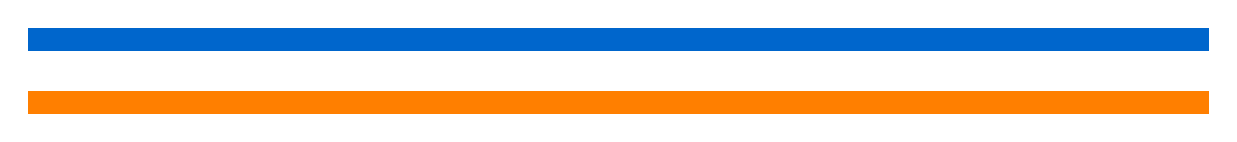
\begin{tikzpicture}
            \fill[primaryBlue] (0,0) rectangle (15,0.3);
            \fill[accentOrange] (0,-0.5) rectangle (15,-0.8);
        \end{tikzpicture}
        
        \vspace{1cm}
        
        {\Huge\bfseries\color{primaryBlue} SavoyConnect Database Schema}
        
        \vspace{0.5cm}
        
        {\LARGE\bfseries Part 7: Tables 61-70}
        
        \vspace{0.5cm}
        
        {\Large Analytics, Activity Logs, Search \& Administration}
        
        \vspace{2cm}
        
        \begin{tcolorbox}[colback=primaryBlue!10,colframe=primaryBlue,arc=3mm,boxrule=1mm,width=0.8\textwidth]
            \centering
            \textbf{\large Document Information}
            
            \vspace{0.3cm}
            
            \begin{tabular}{ll}
                \textbf{Project:} & SavoyConnect E-Commerce Platform \\
                \textbf{Database:} & MySQL 8.0+ \\
                \textbf{Total Tables:} & 80 tables \\
                \textbf{This Document:} & Tables 61-70 (10 tables) \\
                \textbf{Version:} & 1.0 \\
                \textbf{Date:} & November 9, 2025 \\
            \end{tabular}
        \end{tcolorbox}
        
        \vfill
        
        {\large Prepared for: Development Team \\
        SavoyConnect Platform}
        
    \end{center}
\end{titlepage}

% Table of Contents
\tableofcontents
\newpage

\section{Analytics \& Tracking}

\subsection{Table 61: page\_views}

\begin{tablebox}{page\_views - Page View Analytics}
\textbf{Purpose:} Tracks all page views and user navigation patterns for analytics.\\
\textbf{Primary Key:} id\\
\textbf{Foreign Keys:} user\_id, session\_id\\
\textbf{Indexes:} user\_id, session\_id, page\_url, created\_at
\end{tablebox}

\begin{longtable}{|p{3.5cm}|p{2.5cm}|p{6cm}|}
\hline
\rowcolor{tableHeader}
\textcolor{white}{\textbf{Column Name}} & \textcolor{white}{\textbf{Data Type}} & \textcolor{white}{\textbf{Constraints \& Description}} \\
\hline
\endfirsthead

\hline
\rowcolor{tableHeader}
\textcolor{white}{\textbf{Column Name}} & \textcolor{white}{\textbf{Data Type}} & \textcolor{white}{\textbf{Constraints \& Description}} \\
\hline
\endhead

id & BIGINT & PRIMARY KEY, AUTO\_INCREMENT \\
\hline
user\_id & BIGINT & FOREIGN KEY, NULL, References users(id) - NULL for anonymous \\
\hline
session\_id & BIGINT & FOREIGN KEY, NULL, References sessions(id) \\
\hline
page\_url & VARCHAR(1000) & NOT NULL, Full page URL visited \\
\hline
page\_path & VARCHAR(500) & NOT NULL, URL path: "/products/123", "/recipes" \\
\hline
page\_title & VARCHAR(500) & NULL, Page title from HTML \\
\hline
page\_category & VARCHAR(100) & NULL, Category: 'product', 'recipe', 'blog', 'checkout' \\
\hline
referrer\_url & VARCHAR(1000) & NULL, Previous page URL \\
\hline
referrer\_domain & VARCHAR(255) & NULL, External referrer domain \\
\hline
utm\_source & VARCHAR(100) & NULL, UTM parameter: 'facebook', 'google', 'email' \\
\hline
utm\_medium & VARCHAR(100) & NULL, UTM parameter: 'cpc', 'social', 'email' \\
\hline
utm\_campaign & VARCHAR(100) & NULL, Campaign name \\
\hline
utm\_content & VARCHAR(100) & NULL, Ad content identifier \\
\hline
utm\_term & VARCHAR(100) & NULL, Search term \\
\hline
device\_type & ENUM & NOT NULL, Values: 'desktop', 'tablet', 'mobile', 'other' \\
\hline
browser & VARCHAR(100) & NULL, Browser name: 'Chrome', 'Safari', 'Firefox' \\
\hline
browser\_version & VARCHAR(50) & NULL, Browser version \\
\hline
operating\_system & VARCHAR(100) & NULL, OS: 'Windows', 'macOS', 'iOS', 'Android' \\
\hline
screen\_resolution & VARCHAR(50) & NULL, Screen size: '1920x1080' \\
\hline
viewport\_size & VARCHAR(50) & NULL, Viewport dimensions \\
\hline
ip\_address & VARCHAR(45) & NULL, User IP address (IPv4/IPv6) \\
\hline
country & VARCHAR(100) & NULL, Country from IP geolocation \\
\hline
city & VARCHAR(100) & NULL, City from IP geolocation \\
\hline
language & VARCHAR(10) & NULL, Browser language: 'en-US', 'bn-BD' \\
\hline
time\_on\_page & INT & NULL, Seconds spent on page \\
\hline
scroll\_depth & INT & NULL, Percentage scrolled 0-100 \\
\hline
is\_bounce & BOOLEAN & NOT NULL, DEFAULT FALSE, Single page session \\
\hline
created\_at & TIMESTAMP & NOT NULL, DEFAULT CURRENT\_TIMESTAMP \\
\hline
\caption{page\_views table structure}
\end{longtable}

\textbf{Relationships:}
\begin{itemize}
    \item Many-to-One: users (user\_id), sessions (session\_id)
\end{itemize}

\textbf{Analytics Use Cases:}
\begin{itemize}
    \item Most visited pages and products
    \item User journey and navigation paths
    \item Conversion funnel analysis
    \item Marketing campaign effectiveness (UTM tracking)
    \item Device and browser usage patterns
    \item Geographic user distribution
    \item Bounce rate and engagement metrics
    \item Page performance optimization
\end{itemize}

\newpage

\subsection{Table 62: user\_activity\_logs}

\begin{tablebox}{user\_activity\_logs - Detailed User Action Logging}
\textbf{Purpose:} Comprehensive audit trail of all user actions and events.\\
\textbf{Primary Key:} id\\
\textbf{Foreign Keys:} user\_id\\
\textbf{Indexes:} user\_id, activity\_type, entity\_type, created\_at
\end{tablebox}

\begin{longtable}{|p{3.5cm}|p{2.5cm}|p{6cm}|}
\hline
\rowcolor{tableHeader}
\textcolor{white}{\textbf{Column Name}} & \textcolor{white}{\textbf{Data Type}} & \textcolor{white}{\textbf{Constraints \& Description}} \\
\hline
\endfirsthead

\hline
\rowcolor{tableHeader}
\textcolor{white}{\textbf{Column Name}} & \textcolor{white}{\textbf{Data Type}} & \textcolor{white}{\textbf{Constraints \& Description}} \\
\hline
\endhead

id & BIGINT & PRIMARY KEY, AUTO\_INCREMENT \\
\hline
user\_id & BIGINT & FOREIGN KEY, NOT NULL, References users(id) ON DELETE CASCADE \\
\hline
activity\_type & ENUM & NOT NULL, Values: 'create', 'read', 'update', 'delete', 'login', 'logout', 'search', 'click', 'share', 'purchase' \\
\hline
entity\_type & VARCHAR(100) & NOT NULL, Table/entity: 'product', 'order', 'recipe', 'review', 'post' \\
\hline
entity\_id & BIGINT & NULL, ID of the affected entity \\
\hline
action\_description & TEXT & NOT NULL, Human-readable action: "Added product to cart", "Published recipe" \\
\hline
old\_values & JSON & NULL, Previous data state (for updates) \\
\hline
new\_values & JSON & NULL, New data state (for creates/updates) \\
\hline
metadata & JSON & NULL, Additional context data \\
\hline
ip\_address & VARCHAR(45) & NULL, User IP address \\
\hline
user\_agent & TEXT & NULL, Full browser user agent string \\
\hline
device\_fingerprint & VARCHAR(255) & NULL, Unique device identifier \\
\hline
session\_id & BIGINT & NULL, Associated session \\
\hline
page\_url & VARCHAR(1000) & NULL, Page where action occurred \\
\hline
referrer\_url & VARCHAR(1000) & NULL, Previous page \\
\hline
geolocation & JSON & NULL, \{"country": "BD", "city": "Dhaka", "lat": 23.8103, "lng": 90.4125\} \\
\hline
duration\_ms & INT & NULL, Time taken for action (milliseconds) \\
\hline
is\_success & BOOLEAN & NOT NULL, DEFAULT TRUE, Action success status \\
\hline
error\_message & TEXT & NULL, Error details if failed \\
\hline
tags & JSON & NULL, Array of tags: ["high\_value", "first\_time", "promotion"] \\
\hline
created\_at & TIMESTAMP & NOT NULL, DEFAULT CURRENT\_TIMESTAMP \\
\hline
\caption{user\_activity\_logs table structure}
\end{longtable}

\textbf{Relationships:}
\begin{itemize}
    \item Many-to-One: users (user\_id)
\end{itemize}

\textbf{Logged Activities:}
\begin{itemize}
    \item \textbf{Account:} Login, logout, profile updates, password changes
    \item \textbf{Shopping:} Product views, add to cart, checkout, purchases
    \item \textbf{Content:} Recipe views, saves, tries, posts, comments
    \item \textbf{Social:} Follows, likes, shares, messages
    \item \textbf{Reviews:} Write, edit, delete reviews
    \item \textbf{Searches:} Search queries and filters applied
    \item \textbf{Settings:} Preference changes, notification settings
\end{itemize}

\textbf{Data Retention:}
\begin{itemize}
    \item Keep last 90 days for active analysis
    \item Archive older data to cold storage
    \item Anonymize data after 1 year
    \item GDPR compliance: export/delete on request
\end{itemize}

\newpage

\subsection{Table 63: search\_queries}

\begin{tablebox}{search\_queries - Search Query Tracking}
\textbf{Purpose:} Tracks all search queries for analytics and search optimization.\\
\textbf{Primary Key:} id\\
\textbf{Foreign Keys:} user\_id\\
\textbf{Indexes:} user\_id, search\_term, search\_category, created\_at
\end{tablebox}

\begin{longtable}{|p{3.5cm}|p{2.5cm}|p{6cm}|}
\hline
\rowcolor{tableHeader}
\textcolor{white}{\textbf{Column Name}} & \textcolor{white}{\textbf{Data Type}} & \textcolor{white}{\textbf{Constraints \& Description}} \\
\hline
\endfirsthead

\hline
\rowcolor{tableHeader}
\textcolor{white}{\textbf{Column Name}} & \textcolor{white}{\textbf{Data Type}} & \textcolor{white}{\textbf{Constraints \& Description}} \\
\hline
\endhead

id & BIGINT & PRIMARY KEY, AUTO\_INCREMENT \\
\hline
user\_id & BIGINT & FOREIGN KEY, NULL, References users(id) - NULL for anonymous \\
\hline
search\_term & VARCHAR(500) & NOT NULL, Raw search query \\
\hline
search\_term\_normalized & VARCHAR(500) & NOT NULL, Lowercase, trimmed version \\
\hline
search\_category & ENUM & NOT NULL, DEFAULT 'all', Values: 'all', 'products', 'recipes', 'blogs', 'users' \\
\hline
search\_type & ENUM & NOT NULL, DEFAULT 'text', Values: 'text', 'voice', 'image', 'barcode' \\
\hline
filters\_applied & JSON & NULL, Filters: \{"category": "dairy", "price\_max": 500\} \\
\hline
sort\_by & VARCHAR(50) & NULL, Sort option: 'relevance', 'price\_asc', 'rating' \\
\hline
results\_count & INT & NOT NULL, DEFAULT 0, Number of results returned \\
\hline
results\_shown & INT & NULL, Results displayed to user \\
\hline
page\_number & INT & NOT NULL, DEFAULT 1, Pagination page viewed \\
\hline
results\_clicked & INT & NOT NULL, DEFAULT 0, Number of results clicked \\
\hline
first\_click\_position & INT & NULL, Position of first clicked result \\
\hline
time\_to\_first\_click & INT & NULL, Milliseconds to first click \\
\hline
session\_id & BIGINT & NULL, Search session identifier \\
\hline
has\_results & BOOLEAN & NOT NULL, Whether any results found \\
\hline
is\_corrected & BOOLEAN & NOT NULL, DEFAULT FALSE, Query auto-corrected \\
\hline
corrected\_term & VARCHAR(500) & NULL, Suggested correction \\
\hline
suggestions\_shown & JSON & NULL, Auto-complete suggestions displayed \\
\hline
device\_type & ENUM & NOT NULL, Values: 'desktop', 'tablet', 'mobile', 'other' \\
\hline
search\_duration\_ms & INT & NULL, Time to return results (milliseconds) \\
\hline
led\_to\_purchase & BOOLEAN & NOT NULL, DEFAULT FALSE, Resulted in order \\
\hline
order\_id & BIGINT & NULL, Associated order if purchased \\
\hline
created\_at & TIMESTAMP & NOT NULL, DEFAULT CURRENT\_TIMESTAMP \\
\hline
\caption{search\_queries table structure}
\end{longtable}

\textbf{Relationships:}
\begin{itemize}
    \item Many-to-One: users (user\_id)
    \item One-to-Many: search\_results
\end{itemize}

\textbf{Search Analytics:}
\begin{itemize}
    \item Top search terms and trending queries
    \item Zero-result searches (improve catalog/SEO)
    \item Search-to-purchase conversion rate
    \item Average results clicked per search
    \item Search performance optimization
    \item Auto-complete effectiveness
    \item Voice search accuracy
    \item User search patterns and preferences
\end{itemize}

\newpage

\subsection{Table 64: search\_results}

\begin{tablebox}{search\_results - Search Result Click Tracking}
\textbf{Purpose:} Tracks individual search result clicks and ranking performance.\\
\textbf{Primary Key:} id\\
\textbf{Foreign Keys:} search\_query\_id, product\_id\\
\textbf{Indexes:} search\_query\_id, product\_id, position
\end{tablebox}

\begin{longtable}{|p{3.5cm}|p{2.5cm}|p{6cm}|}
\hline
\rowcolor{tableHeader}
\textcolor{white}{\textbf{Column Name}} & \textcolor{white}{\textbf{Data Type}} & \textcolor{white}{\textbf{Constraints \& Description}} \\
\hline
\endfirsthead

\hline
\rowcolor{tableHeader}
\textcolor{white}{\textbf{Column Name}} & \textcolor{white}{\textbf{Data Type}} & \textcolor{white}{\textbf{Constraints \& Description}} \\
\hline
\endhead

id & BIGINT & PRIMARY KEY, AUTO\_INCREMENT \\
\hline
search\_query\_id & BIGINT & FOREIGN KEY, NOT NULL, References search\_queries(id) ON DELETE CASCADE \\
\hline
result\_type & ENUM & NOT NULL, Values: 'product', 'recipe', 'blog', 'user', 'category' \\
\hline
result\_id & BIGINT & NOT NULL, ID of the result entity \\
\hline
product\_id & BIGINT & FOREIGN KEY, NULL, References products(id) - if result is product \\
\hline
position & INT & NOT NULL, Result rank position (1-indexed) \\
\hline
relevance\_score & DECIMAL(5, 4) & NULL, Search engine relevance score 0-1 \\
\hline
was\_clicked & BOOLEAN & NOT NULL, DEFAULT FALSE, Whether user clicked this result \\
\hline
clicked\_at & TIMESTAMP & NULL, When result was clicked \\
\hline
time\_to\_click & INT & NULL, Milliseconds from results shown to click \\
\hline
dwell\_time & INT & NULL, Time spent on result page (seconds) \\
\hline
returned\_to\_results & BOOLEAN & NOT NULL, DEFAULT FALSE, User came back to search results \\
\hline
added\_to\_cart & BOOLEAN & NOT NULL, DEFAULT FALSE, Product added to cart \\
\hline
purchased & BOOLEAN & NOT NULL, DEFAULT FALSE, Product purchased \\
\hline
created\_at & TIMESTAMP & NOT NULL, DEFAULT CURRENT\_TIMESTAMP \\
\hline
\caption{search\_results table structure}
\end{longtable}

\textbf{Relationships:}
\begin{itemize}
    \item Many-to-One: search\_queries (search\_query\_id), products (product\_id)
\end{itemize}

\textbf{Click-Through Analysis:}
\begin{itemize}
    \item CTR by result position (position bias)
    \item Result relevance optimization
    \item Ranking algorithm tuning
    \item A/B testing search algorithms
    \item Personalization effectiveness
    \item Zero-click vs. click searches
    \item Search-to-cart conversion by position
\end{itemize}

\newpage

\subsection{Table 65: click\_tracking}

\begin{tablebox}{click\_tracking - Element Click Tracking}
\textbf{Purpose:} Tracks clicks on UI elements, buttons, and CTAs for UX optimization.\\
\textbf{Primary Key:} id\\
\textbf{Foreign Keys:} user\_id\\
\textbf{Indexes:} user\_id, element\_id, element\_type, created\_at
\end{tablebox}

\begin{longtable}{|p{3.5cm}|p{2.5cm}|p{6cm}|}
\hline
\rowcolor{tableHeader}
\textcolor{white}{\textbf{Column Name}} & \textcolor{white}{\textbf{Data Type}} & \textcolor{white}{\textbf{Constraints \& Description}} \\
\hline
\endfirsthead

\hline
\rowcolor{tableHeader}
\textcolor{white}{\textbf{Column Name}} & \textcolor{white}{\textbf{Data Type}} & \textcolor{white}{\textbf{Constraints \& Description}} \\
\hline
\endhead

id & BIGINT & PRIMARY KEY, AUTO\_INCREMENT \\
\hline
user\_id & BIGINT & FOREIGN KEY, NULL, References users(id) - NULL for anonymous \\
\hline
session\_id & BIGINT & NULL, Associated session \\
\hline
element\_id & VARCHAR(255) & NOT NULL, HTML element ID or tracking identifier \\
\hline
element\_type & ENUM & NOT NULL, Values: 'button', 'link', 'banner', 'card', 'cta', 'image', 'video', 'form', 'other' \\
\hline
element\_text & VARCHAR(500) & NULL, Button/link text content \\
\hline
element\_category & VARCHAR(100) & NULL, Category: 'navigation', 'product', 'checkout', 'social' \\
\hline
page\_url & VARCHAR(1000) & NOT NULL, Page where click occurred \\
\hline
page\_section & VARCHAR(100) & NULL, Section: 'header', 'sidebar', 'footer', 'hero', 'product\_grid' \\
\hline
target\_url & VARCHAR(1000) & NULL, Destination URL (for links) \\
\hline
position\_x & INT & NULL, Click X coordinate \\
\hline
position\_y & INT & NULL, Click Y coordinate \\
\hline
viewport\_width & INT & NULL, Browser viewport width \\
\hline
viewport\_height & INT & NULL, Browser viewport height \\
\hline
scroll\_position & INT & NULL, Vertical scroll position \\
\hline
is\_external & BOOLEAN & NOT NULL, DEFAULT FALSE, External link click \\
\hline
is\_conversion & BOOLEAN & NOT NULL, DEFAULT FALSE, Conversion-related click \\
\hline
campaign\_id & BIGINT & NULL, Associated marketing campaign \\
\hline
ab\_test\_variant & VARCHAR(50) & NULL, A/B test variant identifier \\
\hline
device\_type & ENUM & NOT NULL, Values: 'desktop', 'tablet', 'mobile', 'other' \\
\hline
metadata & JSON & NULL, Additional tracking data \\
\hline
created\_at & TIMESTAMP & NOT NULL, DEFAULT CURRENT\_TIMESTAMP \\
\hline
\caption{click\_tracking table structure}
\end{longtable}

\textbf{Relationships:}
\begin{itemize}
    \item Many-to-One: users (user\_id)
\end{itemize}

\textbf{UX Optimization Use Cases:}
\begin{itemize}
    \item Heatmap generation (click density)
    \item CTA effectiveness analysis
    \item Button placement optimization
    \item Banner and promotion click-through rates
    \item Navigation pattern analysis
    \item Mobile vs. desktop interaction differences
    \item A/B test winner determination
    \item Conversion funnel drop-off points
\end{itemize}

\newpage

\subsection{Table 66: cart\_analytics}

\begin{tablebox}{cart\_analytics - Shopping Cart Analytics}
\textbf{Purpose:} Tracks cart events for abandonment analysis and optimization.\\
\textbf{Primary Key:} id\\
\textbf{Foreign Keys:} user\_id, product\_id\\
\textbf{Indexes:} user\_id, product\_id, event\_type, created\_at
\end{tablebox}

\begin{longtable}{|p{3.5cm}|p{2.5cm}|p{6cm}|}
\hline
\rowcolor{tableHeader}
\textcolor{white}{\textbf{Column Name}} & \textcolor{white}{\textbf{Data Type}} & \textcolor{white}{\textbf{Constraints \& Description}} \\
\hline
\endfirsthead

\hline
\rowcolor{tableHeader}
\textcolor{white}{\textbf{Column Name}} & \textcolor{white}{\textbf{Data Type}} & \textcolor{white}{\textbf{Constraints \& Description}} \\
\hline
\endhead

id & BIGINT & PRIMARY KEY, AUTO\_INCREMENT \\
\hline
user\_id & BIGINT & FOREIGN KEY, NULL, References users(id) - NULL for anonymous \\
\hline
session\_id & BIGINT & NULL, Session identifier \\
\hline
event\_type & ENUM & NOT NULL, Values: 'add', 'remove', 'update\_quantity', 'view', 'checkout\_start', 'checkout\_complete', 'abandon' \\
\hline
product\_id & BIGINT & FOREIGN KEY, NOT NULL, References products(id) \\
\hline
product\_name & VARCHAR(255) & NOT NULL, Product name snapshot \\
\hline
product\_price & DECIMAL(10, 2) & NOT NULL, Price at time of event \\
\hline
quantity & INT & NOT NULL, DEFAULT 1, Quantity in cart \\
\hline
quantity\_change & INT & NULL, Change amount (+ or -) \\
\hline
cart\_total\_items & INT & NOT NULL, Total items in cart \\
\hline
cart\_total\_value & DECIMAL(10, 2) & NOT NULL, Total cart value \\
\hline
cart\_age\_minutes & INT & NULL, Minutes since first item added \\
\hline
page\_url & VARCHAR(1000) & NULL, Page where event occurred \\
\hline
referrer\_source & VARCHAR(255) & NULL, How user arrived: 'search', 'product\_page', 'recommendation' \\
\hline
discount\_applied & DECIMAL(10, 2) & NOT NULL, DEFAULT 0.00, Discount amount \\
\hline
promotion\_code & VARCHAR(100) & NULL, Applied promotion code \\
\hline
device\_type & ENUM & NOT NULL, Values: 'desktop', 'tablet', 'mobile', 'other' \\
\hline
is\_guest & BOOLEAN & NOT NULL, Guest user flag \\
\hline
led\_to\_purchase & BOOLEAN & NOT NULL, DEFAULT FALSE, Resulted in order \\
\hline
order\_id & BIGINT & NULL, Order ID if purchased \\
\hline
abandonment\_reason & VARCHAR(255) & NULL, Reason if abandoned: 'high\_price', 'shipping\_cost', 'out\_of\_stock' \\
\hline
metadata & JSON & NULL, Additional context data \\
\hline
created\_at & TIMESTAMP & NOT NULL, DEFAULT CURRENT\_TIMESTAMP \\
\hline
\caption{cart\_analytics table structure}
\end{longtable}

\textbf{Relationships:}
\begin{itemize}
    \item Many-to-One: users (user\_id), products (product\_id)
\end{itemize}

\textbf{Cart Abandonment Analysis:}
\begin{itemize}
    \item Cart abandonment rate by stage
    \item Most abandoned products
    \item Average cart value at abandonment
    \item Time to abandonment patterns
    \item Price sensitivity analysis
    \item Shipping cost impact on abandonment
    \item Mobile vs. desktop abandonment rates
    \item Recovery email effectiveness
\end{itemize}

\textbf{Optimization Strategies:}
\begin{itemize}
    \item Send cart recovery emails after 1 hour, 24 hours, 3 days
    \item Offer limited-time discounts for abandoned carts
    \item Highlight free shipping thresholds
    \item Show low stock warnings for abandoned items
    \item Simplify checkout process for high-abandonment steps
\end{itemize}

\newpage

\section{Performance \& System}

\subsection{Table 67: conversion\_tracking}

\begin{tablebox}{conversion\_tracking - Conversion Event Tracking}
\textbf{Purpose:} Tracks conversion events and marketing attribution.\\
\textbf{Primary Key:} id\\
\textbf{Foreign Keys:} user\_id, order\_id\\
\textbf{Indexes:} user\_id, order\_id, conversion\_type, created\_at
\end{tablebox}

\begin{longtable}{|p{3.5cm}|p{2.5cm}|p{6cm}|}
\hline
\rowcolor{tableHeader}
\textcolor{white}{\textbf{Column Name}} & \textcolor{white}{\textbf{Data Type}} & \textcolor{white}{\textbf{Constraints \& Description}} \\
\hline
\endfirsthead

\hline
\rowcolor{tableHeader}
\textcolor{white}{\textbf{Column Name}} & \textcolor{white}{\textbf{Data Type}} & \textcolor{white}{\textbf{Constraints \& Description}} \\
\hline
\endhead

id & BIGINT & PRIMARY KEY, AUTO\_INCREMENT \\
\hline
user\_id & BIGINT & FOREIGN KEY, NULL, References users(id) \\
\hline
session\_id & BIGINT & NULL, Session where conversion occurred \\
\hline
conversion\_type & ENUM & NOT NULL, Values: 'purchase', 'signup', 'subscription', 'referral', 'recipe\_publish', 'review\_post', 'social\_share', 'app\_download' \\
\hline
conversion\_value & DECIMAL(10, 2) & NOT NULL, DEFAULT 0.00, Monetary value \\
\hline
order\_id & BIGINT & FOREIGN KEY, NULL, References orders(id) \\
\hline
product\_ids & JSON & NULL, Array of product IDs involved \\
\hline
attribution\_model & ENUM & NOT NULL, DEFAULT 'last\_click', Values: 'last\_click', 'first\_click', 'linear', 'time\_decay', 'position\_based' \\
\hline
first\_touch\_source & VARCHAR(100) & NULL, First interaction source \\
\hline
first\_touch\_medium & VARCHAR(100) & NULL, First interaction medium \\
\hline
first\_touch\_campaign & VARCHAR(100) & NULL, First campaign \\
\hline
first\_touch\_date & TIMESTAMP & NULL, First touchpoint date \\
\hline
last\_touch\_source & VARCHAR(100) & NULL, Last interaction source \\
\hline
last\_touch\_medium & VARCHAR(100) & NULL, Last interaction medium \\
\hline
last\_touch\_campaign & VARCHAR(100) & NULL, Last campaign \\
\hline
last\_touch\_date & TIMESTAMP & NULL, Last touchpoint date \\
\hline
touchpoint\_count & INT & NOT NULL, DEFAULT 1, Number of touchpoints \\
\hline
customer\_journey & JSON & NULL, Full journey: [\{"source": "facebook", "date": "2025-01-15"\}] \\
\hline
days\_to\_conversion & INT & NULL, Days from first touch to conversion \\
\hline
device\_type & ENUM & NOT NULL, Values: 'desktop', 'tablet', 'mobile', 'other' \\
\hline
is\_new\_customer & BOOLEAN & NOT NULL, First purchase flag \\
\hline
revenue\_attributed & DECIMAL(10, 2) & NOT NULL, DEFAULT 0.00, Revenue credited to campaign \\
\hline
cost\_per\_conversion & DECIMAL(10, 2) & NULL, Marketing cost for this conversion \\
\hline
roi & DECIMAL(10, 2) & NULL, Return on investment \\
\hline
created\_at & TIMESTAMP & NOT NULL, DEFAULT CURRENT\_TIMESTAMP \\
\hline
\caption{conversion\_tracking table structure}
\end{longtable}

\textbf{Relationships:}
\begin{itemize}
    \item Many-to-One: users (user\_id), orders (order\_id)
\end{itemize}

\textbf{Attribution Models:}
\begin{itemize}
    \item \textbf{Last Click:} 100\% credit to last touchpoint
    \item \textbf{First Click:} 100\% credit to first touchpoint
    \item \textbf{Linear:} Equal credit across all touchpoints
    \item \textbf{Time Decay:} More credit to recent touchpoints
    \item \textbf{Position-Based:} 40\% first, 40\% last, 20\% middle
\end{itemize}

\textbf{Marketing Analytics:}
\begin{itemize}
    \item Campaign ROI calculation
    \item Channel effectiveness comparison
    \item Customer journey analysis
    \item Multi-touch attribution
    \item Time-to-conversion metrics
    \item New vs. returning customer value
\end{itemize}

\newpage

\subsection{Table 68: admin\_users}

\begin{tablebox}{admin\_users - Administrative User Accounts}
\textbf{Purpose:} Stores admin and staff user accounts with enhanced security.\\
\textbf{Primary Key:} id\\
\textbf{Foreign Keys:} role\_id\\
\textbf{Indexes:} email (unique), username (unique), role\_id, status
\end{tablebox}

\begin{longtable}{|p{3.5cm}|p{2.5cm}|p{6cm}|}
\hline
\rowcolor{tableHeader}
\textcolor{white}{\textbf{Column Name}} & \textcolor{white}{\textbf{Data Type}} & \textcolor{white}{\textbf{Constraints \& Description}} \\
\hline
\endfirsthead

\hline
\rowcolor{tableHeader}
\textcolor{white}{\textbf{Column Name}} & \textcolor{white}{\textbf{Data Type}} & \textcolor{white}{\textbf{Constraints \& Description}} \\
\hline
\endhead

id & BIGINT & PRIMARY KEY, AUTO\_INCREMENT \\
\hline
username & VARCHAR(100) & UNIQUE, NOT NULL, Admin username \\
\hline
email & VARCHAR(255) & UNIQUE, NOT NULL, Admin email \\
\hline
password\_hash & VARCHAR(255) & NOT NULL, Hashed password \\
\hline
full\_name & VARCHAR(255) & NOT NULL, Full name \\
\hline
role\_id & BIGINT & FOREIGN KEY, NOT NULL, References admin\_roles(id) \\
\hline
phone & VARCHAR(20) & NULL, Contact phone \\
\hline
department & VARCHAR(100) & NULL, Department: 'Operations', 'Support', 'Marketing', 'Tech' \\
\hline
status & ENUM & NOT NULL, DEFAULT 'active', Values: 'active', 'inactive', 'suspended', 'locked' \\
\hline
two\_factor\_enabled & BOOLEAN & NOT NULL, DEFAULT FALSE, 2FA enabled flag \\
\hline
two\_factor\_secret & VARCHAR(255) & NULL, TOTP secret key \\
\hline
backup\_codes & JSON & NULL, Array of backup codes (hashed) \\
\hline
last\_login\_at & TIMESTAMP & NULL, Last successful login \\
\hline
last\_login\_ip & VARCHAR(45) & NULL, Last login IP address \\
\hline
login\_attempts & INT & NOT NULL, DEFAULT 0, Failed login count \\
\hline
locked\_until & TIMESTAMP & NULL, Account locked until timestamp \\
\hline
password\_changed\_at & TIMESTAMP & NULL, Last password change \\
\hline
password\_expires\_at & TIMESTAMP & NULL, Password expiration date \\
\hline
must\_change\_password & BOOLEAN & NOT NULL, DEFAULT FALSE, Force password change \\
\hline
session\_timeout & INT & NOT NULL, DEFAULT 3600, Session timeout in seconds \\
\hline
ip\_whitelist & JSON & NULL, Allowed IP addresses \\
\hline
permissions\_override & JSON & NULL, Special permissions beyond role \\
\hline
notes & TEXT & NULL, Admin notes \\
\hline
created\_by & BIGINT & NULL, Admin who created this account \\
\hline
created\_at & TIMESTAMP & NOT NULL, DEFAULT CURRENT\_TIMESTAMP \\
\hline
updated\_at & TIMESTAMP & NOT NULL, DEFAULT CURRENT\_TIMESTAMP ON UPDATE CURRENT\_TIMESTAMP \\
\hline
deleted\_at & TIMESTAMP & NULL, Soft delete timestamp \\
\hline
\caption{admin\_users table structure}
\end{longtable}

\textbf{Relationships:}
\begin{itemize}
    \item Many-to-One: admin\_roles (role\_id)
    \item One-to-Many: admin\_activity\_logs
\end{itemize}

\textbf{Security Features:}
\begin{itemize}
    \item Mandatory 2FA for sensitive roles (Admin, Finance)
    \item Password expiration every 90 days
    \item Account lockout after 5 failed attempts (30 min lockout)
    \item IP whitelisting for critical operations
    \item Session timeout enforcement
    \item Audit trail of all admin actions
    \item Role-based access control (RBAC)
\end{itemize}

\newpage

\subsection{Table 69: admin\_roles}

\begin{tablebox}{admin\_roles - Admin Role Definitions}
\textbf{Purpose:} Defines administrative roles with permission sets.\\
\textbf{Primary Key:} id\\
\textbf{Indexes:} role\_key (unique)
\end{tablebox}

\begin{longtable}{|p{3.5cm}|p{2.5cm}|p{6cm}|}
\hline
\rowcolor{tableHeader}
\textcolor{white}{\textbf{Column Name}} & \textcolor{white}{\textbf{Data Type}} & \textcolor{white}{\textbf{Constraints \& Description}} \\
\hline
\endfirsthead

\hline
\rowcolor{tableHeader}
\textcolor{white}{\textbf{Column Name}} & \textcolor{white}{\textbf{Data Type}} & \textcolor{white}{\textbf{Constraints \& Description}} \\
\hline
\endhead

id & BIGINT & PRIMARY KEY, AUTO\_INCREMENT \\
\hline
role\_key & VARCHAR(100) & UNIQUE, NOT NULL, Role identifier: 'super\_admin', 'admin', 'manager', 'support' \\
\hline
role\_name & VARCHAR(255) & NOT NULL, Display name: 'Super Admin', 'Content Manager', 'Support Agent' \\
\hline
description & TEXT & NULL, Role description \\
\hline
permission\_level & INT & NOT NULL, DEFAULT 0, Hierarchical level 0-100 (higher = more access) \\
\hline
permissions & JSON & NOT NULL, Permission array: ["users.view", "users.edit", "orders.view"] \\
\hline
can\_create\_users & BOOLEAN & NOT NULL, DEFAULT FALSE, Create user permission \\
\hline
can\_delete\_users & BOOLEAN & NOT NULL, DEFAULT FALSE, Delete user permission \\
\hline
can\_manage\_products & BOOLEAN & NOT NULL, DEFAULT FALSE, Product management \\
\hline
can\_manage\_orders & BOOLEAN & NOT NULL, DEFAULT FALSE, Order management \\
\hline
can\_manage\_content & BOOLEAN & NOT NULL, DEFAULT FALSE, Content management \\
\hline
can\_view\_analytics & BOOLEAN & NOT NULL, DEFAULT FALSE, Analytics access \\
\hline
can\_manage\_promotions & BOOLEAN & NOT NULL, DEFAULT FALSE, Promotion management \\
\hline
can\_manage\_settings & BOOLEAN & NOT NULL, DEFAULT FALSE, System settings \\
\hline
can\_access\_api & BOOLEAN & NOT NULL, DEFAULT FALSE, API access \\
\hline
can\_export\_data & BOOLEAN & NOT NULL, DEFAULT FALSE, Data export permission \\
\hline
max\_discount\_percentage & DECIMAL(5, 2) & NULL, Max discount they can apply \\
\hline
max\_refund\_amount & DECIMAL(10, 2) & NULL, Max refund they can authorize \\
\hline
requires\_two\_factor & BOOLEAN & NOT NULL, DEFAULT FALSE, Mandatory 2FA \\
\hline
is\_active & BOOLEAN & NOT NULL, DEFAULT TRUE, Role active status \\
\hline
created\_at & TIMESTAMP & NOT NULL, DEFAULT CURRENT\_TIMESTAMP \\
\hline
updated\_at & TIMESTAMP & NOT NULL, DEFAULT CURRENT\_TIMESTAMP ON UPDATE CURRENT\_TIMESTAMP \\
\hline
\caption{admin\_roles table structure}
\end{longtable}

\textbf{Relationships:}
\begin{itemize}
    \item One-to-Many: admin\_users
\end{itemize}

\textbf{Predefined Roles:}
\begin{itemize}
    \item \textbf{Super Admin (Level 100):} Full system access, manage admins
    \item \textbf{Admin (Level 80):} Most operations, limited admin management
    \item \textbf{Operations Manager (Level 60):} Orders, inventory, delivery
    \item \textbf{Content Manager (Level 50):} Products, recipes, blogs
    \item \textbf{Marketing Manager (Level 50):} Promotions, campaigns, analytics
    \item \textbf{Customer Support (Level 30):} View orders, manage tickets, basic refunds
    \item \textbf{Analyst (Level 20):} Read-only analytics and reports
    \item \textbf{Viewer (Level 10):} Read-only dashboard access
\end{itemize}

\textbf{Permission Examples:}
\begin{verbatim}
{
  "users": ["view", "edit", "delete"],
  "orders": ["view", "edit", "cancel", "refund"],
  "products": ["view", "edit", "create", "delete"],
  "analytics": ["view", "export"],
  "settings": ["view", "edit"]
}
\end{verbatim}

\newpage

\subsection{Table 70: admin\_activity\_logs}

\begin{tablebox}{admin\_activity\_logs - Admin Action Audit Trail}
\textbf{Purpose:} Complete audit log of all administrative actions for security and compliance.\\
\textbf{Primary Key:} id\\
\textbf{Foreign Keys:} admin\_user\_id\\
\textbf{Indexes:} admin\_user\_id, action\_type, entity\_type, created\_at
\end{tablebox}

\begin{longtable}{|p{3.5cm}|p{2.5cm}|p{6cm}|}
\hline
\rowcolor{tableHeader}
\textcolor{white}{\textbf{Column Name}} & \textcolor{white}{\textbf{Data Type}} & \textcolor{white}{\textbf{Constraints \& Description}} \\
\hline
\endfirsthead

\hline
\rowcolor{tableHeader}
\textcolor{white}{\textbf{Column Name}} & \textcolor{white}{\textbf{Data Type}} & \textcolor{white}{\textbf{Constraints \& Description}} \\
\hline
\endhead

id & BIGINT & PRIMARY KEY, AUTO\_INCREMENT \\
\hline
admin\_user\_id & BIGINT & FOREIGN KEY, NOT NULL, References admin\_users(id) \\
\hline
action\_type & ENUM & NOT NULL, Values: 'create', 'read', 'update', 'delete', 'login', 'logout', 'export', 'import', 'approve', 'reject' \\
\hline
action\_description & TEXT & NOT NULL, Human-readable action \\
\hline
entity\_type & VARCHAR(100) & NOT NULL, Affected entity: 'user', 'order', 'product', 'promotion' \\
\hline
entity\_id & BIGINT & NULL, ID of affected entity \\
\hline
old\_values & JSON & NULL, Data before change \\
\hline
new\_values & JSON & NULL, Data after change \\
\hline
changes\_summary & TEXT & NULL, Summary of changes made \\
\hline
affected\_user\_id & BIGINT & NULL, Customer user affected \\
\hline
ip\_address & VARCHAR(45) & NOT NULL, Admin IP address \\
\hline
user\_agent & TEXT & NULL, Browser/device info \\
\hline
request\_method & VARCHAR(10) & NULL, HTTP method: 'GET', 'POST', 'PUT', 'DELETE' \\
\hline
request\_url & VARCHAR(1000) & NULL, API endpoint or page URL \\
\hline
request\_payload & JSON & NULL, Request data sent \\
\hline
response\_status & INT & NULL, HTTP response code \\
\hline
severity & ENUM & NOT NULL, DEFAULT 'info', Values: 'info', 'warning', 'error', 'critical' \\
\hline
is\_sensitive & BOOLEAN & NOT NULL, DEFAULT FALSE, Sensitive operation flag \\
\hline
requires\_audit\_review & BOOLEAN & NOT NULL, DEFAULT FALSE, Needs compliance review \\
\hline
session\_id & VARCHAR(255) & NULL, Admin session identifier \\
\hline
duration\_ms & INT & NULL, Time taken for action \\
\hline
is\_successful & BOOLEAN & NOT NULL, DEFAULT TRUE, Action success status \\
\hline
error\_message & TEXT & NULL, Error details if failed \\
\hline
tags & JSON & NULL, Tags: ["financial", "pii", "bulk\_operation"] \\
\hline
created\_at & TIMESTAMP & NOT NULL, DEFAULT CURRENT\_TIMESTAMP \\
\hline
\caption{admin\_activity\_logs table structure}
\end{longtable}

\textbf{Relationships:}
\begin{itemize}
    \item Many-to-One: admin\_users (admin\_user\_id)
\end{itemize}

\textbf{Critical Actions Logged:}
\begin{itemize}
    \item \textbf{User Management:} Create, edit, delete, suspend users
    \item \textbf{Financial:} Refunds, discounts, price changes, wallet adjustments
    \item \textbf{Order Management:} Cancel, modify, status changes
    \item \textbf{System Settings:} Configuration changes, feature toggles
    \item \textbf{Content:} Product creation, recipe approval, content moderation
    \item \textbf{Access:} Login, logout, permission changes, role assignments
    \item \textbf{Data Export:} PII exports, bulk data downloads
    \item \textbf{Security:} 2FA changes, password resets, IP whitelist updates
\end{itemize}

\textbf{Compliance \& Security:}
\begin{itemize}
    \item Immutable logs (no delete/edit)
    \item Encrypted storage for sensitive data
    \item Retain logs for 7 years (compliance requirement)
    \item Real-time alerts for suspicious activity
    \item Regular audit reviews for critical operations
    \item PCI-DSS compliance for payment-related actions
    \item GDPR compliance for data access/export
\end{itemize}

\newpage

\section{Summary}

\begin{tcolorbox}[colback=primaryBlue!10,colframe=primaryBlue,arc=3mm,boxrule=1mm]
\textbf{\large Part 7 Complete: Tables 61-70}

\vspace{0.3cm}

This document covers tables 61-70 of the SavoyConnect database schema:

\begin{itemize}
    \item \textbf{Analytics \& Tracking (6 tables):} page\_views, user\_activity\_logs, search\_queries, search\_results, click\_tracking, cart\_analytics
    \item \textbf{Performance \& System (1 table):} conversion\_tracking
    \item \textbf{Administration (3 tables):} admin\_users, admin\_roles, admin\_activity\_logs
\end{itemize}

\vspace{0.3cm}

\textbf{Key Features Implemented:}
\begin{itemize}
    \item Comprehensive page view tracking with UTM parameters and device detection
    \item Detailed user activity logging for audit trails and behavior analysis
    \item Search query analytics with click-through tracking and result optimization
    \item Individual search result performance tracking for ranking improvements
    \item UI element click tracking for heatmaps and UX optimization
    \item Shopping cart event tracking for abandonment analysis
    \item Multi-touch attribution for marketing ROI and conversion tracking
    \item Secure admin user management with 2FA and enhanced security
    \item Role-based access control (RBAC) with granular permissions
    \item Complete admin activity audit logs for compliance and security
\end{itemize}

\vspace{0.3cm}

\textbf{Analytics Capabilities:}
\begin{itemize}
    \item User journey mapping from first touch to conversion
    \item Marketing campaign effectiveness and ROI calculation
    \item Search engine optimization and result relevance tuning
    \item Cart abandonment recovery strategies
    \item Heatmap generation and UX bottleneck identification
    \item Device and browser usage patterns
    \item Geographic user distribution and localization insights
    \item Real-time dashboard metrics and KPI tracking
\end{itemize}

\vspace{0.3cm}

\textbf{Security \& Compliance:}
\begin{itemize}
    \item Immutable audit logs with 7-year retention
    \item PII data encryption and GDPR compliance
    \item PCI-DSS compliance for payment operations
    \item IP whitelisting and session management
    \item Mandatory 2FA for sensitive admin roles
    \item Real-time suspicious activity alerts
    \item Role-based access control with permission hierarchy
\end{itemize}

\vspace{0.3cm}

\textbf{Next Document:} Part 8 will cover tables 71-80 (Final 10 tables: System Configuration, API Management, Email Templates, File Storage, Cron Jobs, Error Logs, and Supporting Tables)

\end{tcolorbox}

\end{document}
